\chapter{Preparation}

\section{Theory}
Commonly two kinds of photodetectors are used. PIN-Photodiodes and Avalanche Photo Diodes (APD).
\subsection{PIN-Photodiode}

\subsection{Avalanche Photo Diode (APD)}



\section{Question 1: Open Circuit Voltage}
The Term (1)
\begin{equation}
 I_{\mathrm{PIN}} = I_{\mathrm{Sat}}\left[\exp\left(\frac{U_{\mathrm{PIN}}}{U_{\mathrm{T}}}\right)-1\right] -I_{\mathrm{pr}}
\label{eq:diode}
\end{equation}
from the experiment description, with $R_{\mathrm{a}}\to\infty(I_{\mathrm{PIN}}\to0)$ can be rearranged to:
\begin{equation}
 I_{\mathrm{pr}} = I_{\mathrm{Sat}}\left[\exp\left(\frac{U_{\mathrm{PIN0}}}{U_{\mathrm{T}}}\right)-1\right]
\end{equation}
and further to:
\begin{equation}
 U_{\mathrm{PIN0}}(I_{\mathrm{pr}}) = U_{\mathrm{T}}\ln\left(\frac{I_{\mathrm{pr}}}{I_{\mathrm{Sat}}}+1\right)
\end{equation}

\section{Question 2: Electrical Power of a PIN Diode}

With $P = R\cdot I^2$, $I_{\mathrm{pr}} = S\cdot P$ and equation \eqref{eq:diode}, the Power of the PIN-diode can be calculated by:
\begin{equation}
 P_{\mathrm{el}} = R_{\mathrm{a}}\cdot\left\{ I_{\mathrm{Sat}}\left[\exp\left(\frac{U_{\mathrm{PIN}}}{U_{\mathrm{T}}}\right)-1\right] -S\cdot P\right\}^2.
\label{eq:power}
\end{equation}
For the Case:
\begin{equation}
 \frac{U_{\mathrm{PIN}}}{U_{\mathrm{T}}} \ll 1 \to \exp\left(\frac{U_{\mathrm{PIN}}}{U_{\mathrm{T}}}\right)\approx1+\frac{U_{\mathrm{PIN}}}{U_{\mathrm{T}}}
\label{eq:vereinfachung}
\end{equation}
equation \eqref{eq:diode} can be simplified to:
%\begin{equation}
%  P_{\mathrm{el}} = R_{\mathrm{a}}\cdot\left\{ I_{\mathrm{Sat}}\cdot\frac{U_{\mathrm{PIN}}}{U_{\mathrm{T}}} -S\cdot P\right\}^2.
%\end{equation}
%
%Because of \eqref{eq:vereinfachung} the primary photo current $S\cdot P$ is dominating. 
\begin{equation}
I_{\mathrm{PIN}} = I_{\mathrm{Sat}}\cdot\frac{U_{\mathrm{PIN}}}{U_{\mathrm{T}}} -S\cdot P
\label{eq:}
\end{equation}
The power $P = U_{\mathrm{PIN}} \cdot I_{\mathrm{PIN}}$ can be maximized  by deriving $P$ by $U_{\mathrm{PIN}}$. That way the voltage for the maximum power can be obtained. 
\begin{equation}
U_{\mathrm{PIN}} = \frac{S\cdot P \cdot U_{\mathrm{T}}}{2\cdot I_{\mathrm{sat}}} 
\label{eq:}
\end{equation}
Inserting this therm into \eqref{eq:diode} the current for the maximum power is

\begin{equation}
I_{\mathrm{PIN}} = - \frac{S \cdot P}{2}
\label{eq:}
\end{equation}

Thus for $R = U/I$ the resistance for the maximum power is

\begin{equation}
R_{\mathrm{max}} = - \frac{U_{\mathrm{T}}}{I_{\mathrm{Sat}}}
\label{eq:}
\end{equation}

For the maximum power then results:
\begin{equation}
 P_{\mathrm{max}}= \frac{S^2\cdot P^2\cdot U_{\mathrm{T}}}{4 \cdot I_{\mathrm{sat}}}
\end{equation}

%\todo{da stimmt irgendwas noch net}

\section{Question 3: Photodetector with Transimpedance Amplifier}

\begin{figure}[h]%
\centering
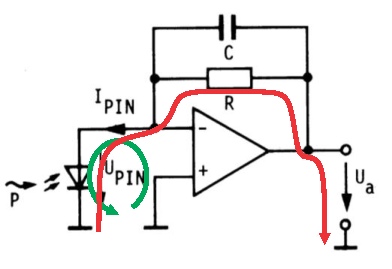
\includegraphics[width=.8\columnwidth]{Grafiken/OPAMP_m.pdf}
\caption{}%
\label{fig:OPAMP}%

\end{figure}

In Figure \ref{fig:OPAMP} with Kirchhoff's second law it can be derived (using the red loop):
\begin{equation}
 - u_{\mathrm{PIN}} - i_{\mathrm{PIN}}\cdot \frac{R}{1+ j\omega RC}+u_{\mathrm{a}} = 0 .
\label{eq:masche1}
\end{equation}
Using
\begin{equation}
 u_{\mathrm{PIN}}=0.
\label{eq:masche2}
\end{equation}
resulting also from Kirchhoff's second law (green loop) you get:
\begin{equation}
 u_{\mathrm{a}} = i_{\mathrm{PIN}}\cdot \frac{R}{1+ j\omega RC}.
\label{eq:ua}
\end{equation}

For the cut-off frequency $f_{\mathrm{3dB}}$ the following condition has to be fulfilled:
\begin{equation}
 \left|\frac{u(f_{\mathrm{3dB}})}{u(0)}\right| = \frac{1}{\sqrt{2}}
\end{equation}
With \eqref{eq:ua} you obtain
\begin{equation}
 \left|\frac{i_{\mathrm{PIN}}\cdot \frac{R}{1+ j2\pi f_{\mathrm{3dB}} RC}}{i_{\mathrm{PIN}}\cdot R}\right| = \frac{1}{\sqrt{2}}
\end{equation}
and further
\begin{equation}
 f_{\mathrm{3dB}} = \frac{\sqrt{2}-1}{2\pi RC} 
\end{equation}

With \eqref{eq:ua}, \eqref{eq:diode},\eqref{eq:masche2} and $I_{\mathrm{pr}}=S\cdot P$ it can be obtained:

\begin{equation}
 u_{\mathrm{a}} =  -S\cdot P\cdot \frac{R}{1+ j\omega RC}
\end{equation}

Because in a stationary case $i$ is proportional to eFg it is also proportional to $P_e$. Here $e$ is the elementary charge, $F$ the active surface and $g$ the optical generation rate.
 
The multiplication in the APD is caused by impact ionization. The ionization probabilities $\beta_i$ and $\alpha_i$ are proportional to $e^{\frac{-W_{\mathrm{ion}}}{W_T}},  W_T=eEl_\mathrm{LO}$. Here $E$ is the electrical field, $l_\mathrm{LO}$ the free path. Therefore $\beta_i$ and $\alpha_i$ are independent of $P$.


Thus for a constant $\omega$, $u_{\mathrm{a}}$ is linearly dependent on the optical power $P$. The proportionality constant is 
\begin{equation}
\zeta = -S\cdot \frac{R}{1+ j\omega RC}.
\label{eq:}
\end{equation}
 
\section{Question 4: APD - Change of light power}

%\begin{equation}
%eFg_{\mathrm{photo}} = \frac{\eta e}{hf_L}P_e\frac{\alpha e^{-\alpha(x+w_a)}}{1-e^{-\alpha w_A}}, \rightarrow eFg_{\mathrm{photo}} \propto P_e.
%\label{eq:}
%\end{equation}
%
%Because in a stationary case $i$ is proportional to eFg it is also proportional to $P_e$. Here $e$ is the elementary charge, $F$ the active surface and $g$ the optical generation rate.
% 
%The multiplication in the APD is caused by impact ionization. The ionization probabilities $\beta_i$ and $\alpha_i$ are proportional to 
%\begin{equation}
%\alpha_i, \beta_i \propto e^{\frac{-W_{\mathrm{ion}}}{W_T}},  W_T=eEl_\mathrm{LO}.
%\label{eq:}
%\end{equation}
%
%
%Here $E$ is the electrical field, $l_\mathrm{LO}$ the free path. Therefore $\beta_i$ and $\alpha_i$ are independent of $P$.
%
%Since $M_0$ is for the stationary case (dP/dt=0)
%\begin{equation}
%M_0=\frac{(\beta_i  -\alpha_i)e^{(\beta_i-\alpha_i)w_L}}{\beta_i - \alpha_i e^{(\beta_i - \alpha_i)w_L}},
%\label{eq:}
%\end{equation}
%$w_L$ is the length of the avalanche-zone, $M_0$ does not depend on $P$.
%with the differential equation
%
%\begin{equation}
%\frac{1}{v_p} \frac{\partial i_p}{\partial t} +\frac{\partial i_p}{\partial x} = eFg_{\mathrm{photo}} 
%\label{eq:}
%\end{equation}
%
%and
%
%\begin{equation}
%\frac{1}{v_n} \frac{\partial i_n}{\partial t} +\frac{\partial i_n}{\partial x} = eFg_{\mathrm{photo}} 
%\label{eq:}
%\end{equation}
%
%follows for $\frac{\partial}{\partial t} = 0$
%
%
%\begin{equation}
%i_p = eFg_{\mathrm{photo}}\cdot x
%\label{eq:}
%\end{equation}
%
%\begin{equation}
%i_n = eFg_{\mathrm{photo}}\cdot x
%\label{eq:}
%\end{equation}
%
%Therefore $i_n$, $i_p$ $\propto P_e$.
%
%At a APD there's an impact ionszation. 
%\begin{equation}
%eFg_{\mathrm{ion}} = \alpha_i i_n + \beta_i i_p
%\label{eq:}
%\end{equation}

The in figure \ref{fig:Q4_APD}\footnote[1]{Source: OKT Experiment 2: Photodiode analysis task-sheet} shown circuit is given.
The APD gets radiated by a power $P$. 
When changing the radiating power to $P + \Delta P$ several things change in the circuit.

The circuit is driven by a constant voltage of $U = 0.9\cdot U_{\mathrm{BR}}$. When changing $P$, $I_{\mathrm{APD}}$ changes proportional to the change of $P$.

A change of $I_{\mathrm{APD}}$ causes a change of the voltage that falls off over $R_{\mathrm{V}}$. Since the driving voltage is constant, the voltage over the APD decreases. Because $M_0$ depends strongly on $U_{\mathrm{APD}}$, $M_0$ decreases as well. 



\begin{figure}%
\centering
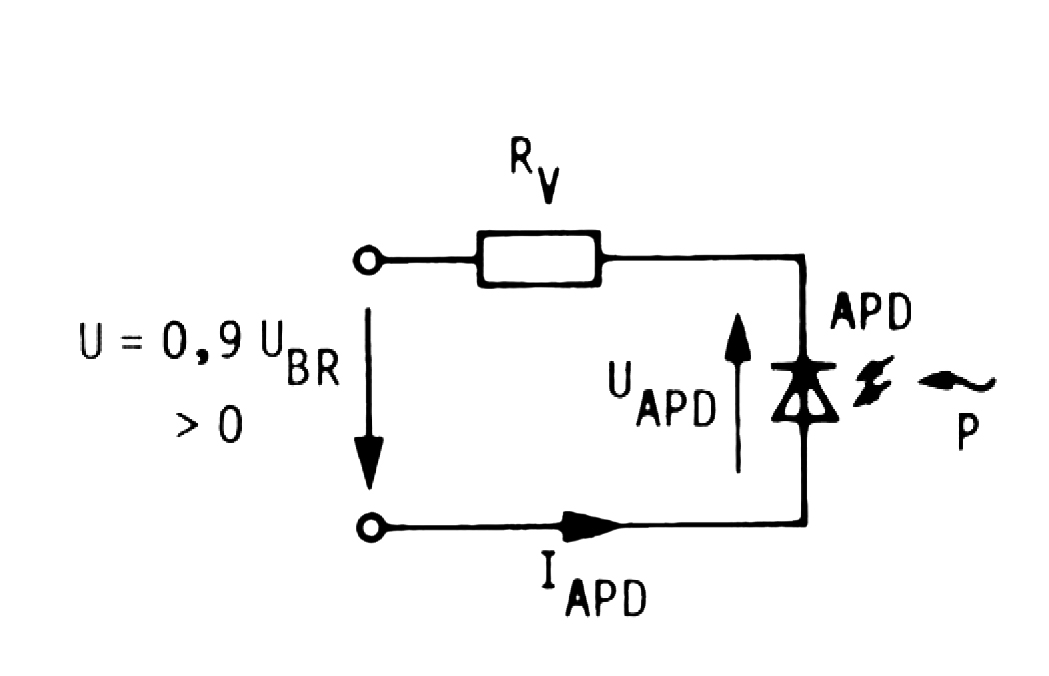
\includegraphics[width=.5\columnwidth]{Grafiken/Q4_APD.jpg}%
\caption{APD with series resistance}%
\label{fig:Q4_APD}%
\end{figure}


